\chapter{Thesis}
\label{cha:Diplomschrift}

\section{The physical Track}

Being able to drive along a simulation of the track is only a partial success. In order to prove successful, the trained algorithm is required to complete multiple runs on a real track using our DeepRacer vehicle. We decided on rebuilding the track used 2018 during the AWS re:Invent.

The circular track starts with a 180° left turn, followed by a right-starting s-curve and continues on with two left turns back to the beginning. With a total width of 7.93 m and length of 5.18 m it impractical to paint it on a single, solid piece.

Before we considered building the track, we painted it on the floor in our robotics laboratory. This was possible due to the floor being solid black, just like the road on the track.

Rather than that we chose to use interlocking foam pieces which are lightweight and easy to store and transport.

\begin{figure}
    \centering
    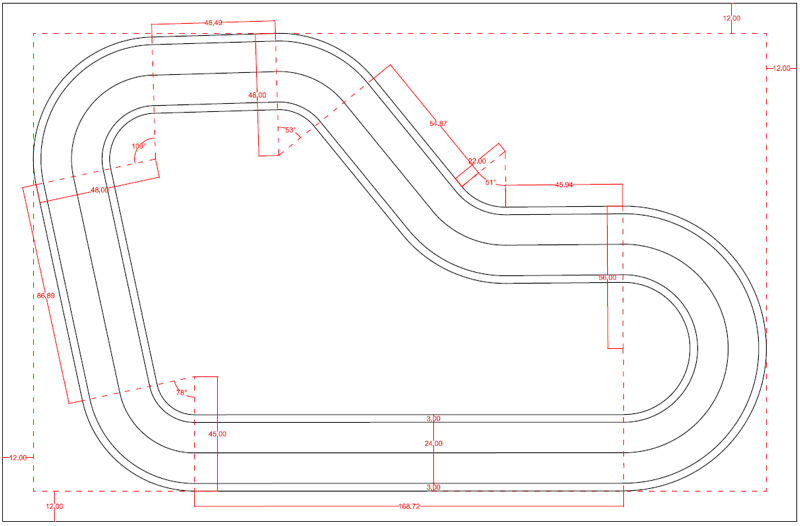
\includegraphics[width=.85\textwidth]{deepracer-track-2018-guideline.png}
    \caption{AWS re:Invent 2018 track}
    \label{fig:track}
\end{figure}

\section{Machine Learning and Autonomous Driving}


 \section{Local Training}
 
 One of the major drawbacks of using the DeepRacer in a learning environment are the costs of training. Amazon offers easy, albeit functionally limited ways of training RL models in their cloud services. This sort of contradicts the intended use, as the DeepRacer is supposed to offer a simple and affordable entry into the ways of machine learning. Below is the pricing table. \footnote{Cited date 2020/08/20}
 \begin{table}
 \caption{Pricing for model training with AWS services.}
 \label{tab:services}
 \centering
 \setlength{\tabcolsep}{5mm}
 \def\arraystretch{1.25}
 \begin{tabular}{|r|r|c|c|c|}
 \hline
 \textbf{service} & \textbf{pricing} \\
 \hline\hline
 training and evaluation & 3.50 US\$ per hour \\
 \hline
 model storage & 0.023 US\$ per GB \\
 \hline
 \end{tabular}
 \end{table}
 In order to circumvent this cost barrier we -- like others before us -- began setting up a training environment on one of the more powerful computers in the robotics lab.
 The setup for local training is available on GitHub \footcite{https://github.com/aws-deepracer-community/deepracer}. In order to function properly the computer had to meet the following requirements:
 \begin{itemize}
 \item A Linux distribution, preferably Ubuntu
 \item NVIDIA grafic processor and proper dirvers
 \item Docker
 \item Python
 \item Minio, a S3 simulator
 \end{itemize}